\documentclass[12pt,letterpaper]{article}
\usepackage[utf8]{inputenc}
\usepackage{listings, float, xcolor}

%----- Configuración del estilo del documento------%
\usepackage{graphicx, fancyhdr, lastpage}
\usepackage{enumitem, pifont, hyperref, ulem}
\usepackage[left=2cm,right=2cm,top=1.8cm,bottom=2.3cm]{geometry}

\pagestyle{fancy}
\fancyhf{}
\rfoot{\textit{Página \thepage \hspace{1pt} de \pageref{LastPage}}}

%------ Paquetes matemáticos básicos --------%
\usepackage{amsmath, amssymb, amsthm}

%------ Personalizar el link al video  --------%
\hypersetup{
  colorlinks=true,
  linkcolor=blue!50!black, % Azul oscuro
  urlcolor=blue!50!black,  % Azul oscuro
  hidelinks % Elimina el recuadro azul
}

\newcommand{\imp}{\rightarrow}

\begin{document}

%------ Encabezado -------- %
\begin{center}
  \begin{minipage}{3cm}
    \begin{center}
      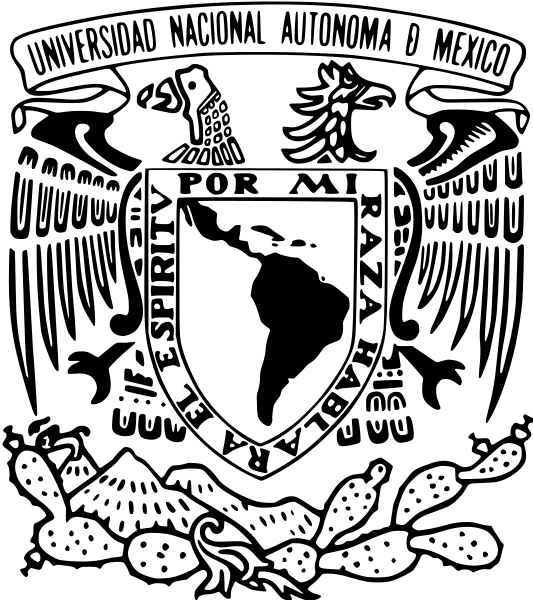
\includegraphics[height=3.4cm]{../unam_logo.png}
    \end{center}
  \end{minipage}\hfill
  \begin{minipage}{10cm}
    \begin{center}
      \textbf{\Large Universidad Nacional Autónoma de México}\\[0.2cm]
      \textbf{\large Facultad de Ciencias}\\[0.2cm]
      \textbf{Organización y Arquitectura de Computadoras 2025-2}\\[0.4cm]
      \textbf{\Large Tarea 01}\\[0.1cm]
      \textbf{Docentes:}\\
      José Galaviz \hspace{1em} Ricardo Pérez \hspace{1em} Ximena Lezama\\[0.3cm]
      \textbf{Autores:}\\
      Fernanda Ramírez Juárez \quad Ianluck Rojo Peña\\[0.2cm]
      \textbf{No. de cuenta:}\\
      321204747 \quad 118005762\\[0.2cm]
      \textbf{Fecha de entrega:} Miércoles 12 de marzo de 2025
    \end{center}
  \end{minipage}\hfill
  \begin{minipage}{3cm}
    \begin{center}
      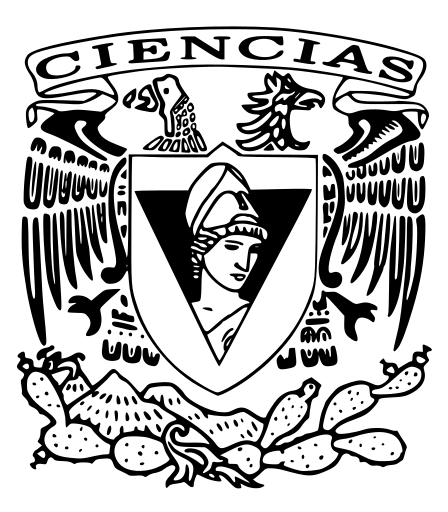
\includegraphics[height=3.4cm]{../fc_logo.png}
    \end{center}
  \end{minipage}
\end{center}

\bigskip
\hrule height 0.1pt
\bigskip

%------ Contenido -------- %
\section*{Preguntas.}

\begin{enumerate}
\item Expresar -31 y +31 en 8 bits en el sistema de complemento a 1.
  \bigskip
  % -- Respuesta -- %

  +31 en binario expresado en 8 bits es $31_{10} = 00011111_2$. Por lo que en complemento a uno para obtener -31 es invertir los bits del n\'{u}mero positivo es decir 31.\\
  Entonces si $31_{10} = 00011111_2$ tenemos que $-31_{10} = 11100000_2$.
  \[
  \therefore \text{En el sistema de complemento a uno en 8 bits, } +31_{10} = 00011111_2 \text{ y} -31_{10} = 11100000.
  \]
  
\item Expresar +13 y -13 en 8 bits en el sistema de complemento a 2.
  \bigskip
  % -- Respuesta -- %

  +13 en binario expresado en 8 bits es $13_{10} = 00001101_2$. Usando el complemento a dos para obtener -13 es invertir los bits de 13 y sumarle un bit.\\
  Invertimos $00001101_2 \imp 11110010_2$ sumamos un bit $11110010_2 + 1 = 11110011_2$
  Entonces si $13_{10} = 00001101_2$ tenemos que $-13_{10} = 11110011_2$.
  \[
  \therefore \text{En el sistema de complemento a dos en 8 bits, } +13_{10} = 00001101_2 \text{ y} -13_{10} = 11110011_2.
  \]
  
\item ¿Cuál es el rango de números representables en complemento a dos con 4 bits?
  \bigskip
  % -- Respuesta -- %

  El rango de números representables en complemento a dos con n bits es de la forma $2^{n-1}$ para los números negativos y $2^{n1} - 1$ para los números positivos.\\
  Así el rango  de nmeros representables en complemento a dos con 4 bits es de
  \[
  -(2^{4-1}),\hspace{3mm} 2^{4-1} - 1] = [-(2^3),\hspace{3mm} 2^{3} - 1] = [-8,\hspace{3mm} 7]
    \]

  \item El número $(10110101)_2$ es un número de 8 bits incluyendo el bit signo en complemento a 2.\\
    Da su equivalente en base decimal.
    \bigskip
    % -- Respuesta -- %

    Para pasarlo miramos el primer digito para saber si es positivo o negativo.
    Si es un 0 es positivo y lo podr\'{i}amos pasar a decimal como un n\'{u}mero binario natural.
    Si es un 1 es negativo y lo tendremos que convertir en binario natural.

    En el caso de $10110101_2$, como el primer d\'{i}gito es un 1, entonces tenemos un negativo y lo tendremos que complementar a dos.
    Para ello vamos recorriendo desde atras hacia delante invirtiendo s\'{o}lo a partir del primer uno.

    De manera que $10110101_2 \imp 01001011_2$ que ser\'{i}a el numero en positivo y ahora lo podemos pasar a decimal como un n\'{u}mero binario natural.
    
    Para hacer esta conversión debemos usar la siguiente f\'{o}rmula:\\
    Si tenemos un número binario $b_{n-1} .... b_1 b_0$ debemos multiplicar cada casilla por su potencia de 2
    Decimal $= b_0 * 2 b^0 + .... b_{n-1} * 2 b^{n-1}$.\\
    En este caso para el binario $01001011_2$:
    
    \begin{center}
      $(0 × 2^7) + (1 × 2^6) + (0 × 2^5) + (0 × 2^4) + (1 × 2^3) + (0 × 2^2) + (1 × 2^1) + (1 × 2^0)$\\
      $(0 × 128) + (0 × 64) + (1 × 32) + (1 × 16) + (0 × 8) + (1 × 4) + (1 × 2) + (1 × 1)$\\
      $= 64 + 8 + 2 + 1 = 75$
    \end{center}

    As\'{i} $01001011_2 = 75_{10}$ pero recordemos que el n\'{u}mero original es negativo pues primero obtuvimos su complemento a dos y luego lo pasamos a binario natural.
    \[
    \therefore \text{El resultado del numero binario } 10110101_2 \text{ en decimal es } -75_{10}
    \]
    
  \item El número $(00110111)_2$ es un número de 8 bits incluyendo el bit signo en complemento a 2.\\
    Da su equivalente en base decimal.
    \bigskip
    % -- Respuesta -- %

    Recordando del ejercicio anterior para pasarlo miramos el primer digito para saber si es positivo o negativo.

    En el caso de $00110111_2$, como el primer d\'{i}gito es un 0, entonces tenemos un positivo y lo pasamos a decimal como un n\'{u}mero binario natural.

    Recordando la f\'{o}rmula:\\
    Si tenemos un número binario $b_{n-1} .... b_1 b_0$ debemos multiplicar cada casilla por su potencia de 2
    Decimal $= b_0 * 2 b^0 + .... b_{n-1} * 2 b^{n-1}$
    En este caso para el binario $00110111_2$:
    
    \begin{center}
      $(0 × 2^7) + (0 × 2^6) + (1 × 2^5) + (1 × 2^4) + (0 × 2^3) + (1 × 2^2) + (1 × 2^1) + (1 × 2^0)$\\
      $(0 × 128) + (0 × 64) + (1 × 32) + (1 × 16) + (0 × 8) + (1 × 4) + (1 × 2) + (1 × 1)$\\
      $= 32 + 16 + 4 + 2 + 1 = 55$
    \end{center}

    \[
    \therefore \text{El resultado del numero binario } 00110111_2 \text{ en decimal es } 55_{10}
    \]
    
  \item Menciona las cuatro unidades funcionales principales de una computadora y describe su funcionamiento.
    \bigskip
    % -- Respuesta -- %

    Las cuatro unidades funcionales principales de una computadora son:
    \begin{enumerate}[label=\arabic*)]
    \item \textbf{Unidad de Control (CU, Control Unit):}
      La Unidad de Control es uno de los componentes más importantes de la CPU y actúa como el "cerebro" de la computadora.\\
      Su principal función es supervisar y coordinar todas las operaciones que se realizan dentro del sistema.\\
      \textit{Funcionamiento:}
      \begin{itemize}
      \item La CU interpreta las instrucciones que forman parte de un programa, las cuales están almacenadas en la memoria.
        Estas instrucciones son traducidas a señales de control que indican a otros componentes qué hacer y en qué momento.
        
      \item Dirige el flujo de datos entre la CPU, la memoria y los dispositivos de entrada/salida, asegurando que cada componente reciba la información necesaria en el orden correcto.
        
      \item Coordina las operaciones de la ALU y gestiona el acceso a la memoria principal para leer o escribir datos.
        
      \item Y cómo se mencionó, la CU es responsable de mantener la sincronización de todas las operaciones, lo que garantiza que la computadora funcione de manera eficiente y sin errores.
      \end{itemize}
      
    \item \textbf{Unidad Aritmético-Lógica (ALU):}
      La ALU es el componente de la CPU encargado de realizar operaciones matemáticas y lógicas, lo que la convierte en el núcleo del procesamiento de datos.
      
      \textit{Funcionamiento:}
      \begin{itemize}
      \item La ALU también realiza operaciones lógicas, como comparaciones entre valores (por ejemplo, determinar si un número es mayor, menor o igual que otro) y operaciones booleanas (AND, OR, NOT).
        Estas operaciones son cruciales para la toma de decisiones dentro de los programas.
        
      \item La ALU trabaja en conjunto con la Unidad de Control, que le indica qué operaciones realizar y le proporciona los datos necesarios desde la memoria.
        
      \item Una vez que la ALU completa una operación, envía los resultados de vuelta a la memoria o a otros componentes para su uso posterior.
      \end{itemize}
      
    \item \textbf{Memoria:}
      La memoria principal permite un acceso rápido a la información que el procesador necesita en tiempo real.\\
      También existen memorias secundarias (discos duros, SSD) que almacenan información de forma permanente.
      La memoria es el componente que permite almacenar tanto las instrucciones de los programas como los datos que se están procesando.\\
      Sin memoria, la computadora no podría ejecutar tareas ni guardar información.
      
      \textit{Funcionamiento:}\\
      \textbf{RAM:}
      \begin{itemize}
      \item La memoria de acceso aleatorio (RAM) es volátil, lo que significa que solo almacena información mientras la computadora está encendida.
        
      \item Proporciona un acceso rápido a los datos que la CPU necesita en tiempo real, lo que permite una ejecución eficiente de los programas.
        
      \item La RAM es esencial para el multitasking, ya que permite que varios programas se ejecuten simultáneamente al almacenar sus datos e instrucciones de manera temporal.
      \end{itemize}
      
      \textbf{Memoria Secundaria:}
      \begin{itemize}
      \item Incluye dispositivos como discos duros (HDD), unidades de estado sólido (SSD) y memorias USB.
        
      \item A diferencia de la RAM, la memoria secundaria es no volátil, lo que significa que retiene la información incluso cuando la computadora está apagada.
        
      \item Se utiliza para almacenar sistemas operativos, aplicaciones, archivos y otros datos de manera permanente.
      \end{itemize}
      
      \textbf{Memoria Caché:}
      \begin{itemize}
      \item Es un tipo de memoria más rápida que la RAM y se encuentra dentro de la CPU.
        
      \item Almacena copias de los datos e instrucciones más utilizados, lo que reduce el tiempo de acceso y mejora el rendimiento del sistema.
      \end{itemize}
      
    \item \textbf{Unidad de Entrada/Salida (I/O, Input/Output):}
      La Unidad de Entrada/Salida es responsable de la comunicación entre la computadora y el mundo exterior.\\
      Permite que los usuarios interactúen con el sistema y que la computadora reciba y envíe información.

      \textit{Funcionamiento:}\\
      \textbf{Dispositivos de Entrada:}
      \begin{itemize}
      \item Estos dispositivos permiten que los usuarios introduzcan datos en la computadora.
        Ejemplos comunes incluyen el teclado, el mouse, los escáneres y los micrófonos.
        
      \item Los datos ingresados se envían a la memoria o a la CPU para su procesamiento.
      \end{itemize}
      
      \textbf{Dispositivos de Salida:}
      \begin{itemize}
      \item Muestran o presentan los resultados del procesamiento de datos.
        Algunos ejemplos son los monitores, las impresoras y los altavoces.
        
      \item Estos dispositivos permiten que los usuarios vean, escuchen o utilicen la información generada por la computadora.
      \end{itemize}
      
      \textbf{Controladores de Entrada/Salida:}
      \begin{itemize}
      \item Son circuitos especializados que gestionan la comunicación entre la CPU y los dispositivos de entrada/salida.
        
      \item Aseguran que los datos se transfieran de manera eficiente y sin errores.
      \end{itemize}
    \end{enumerate}
    \bigskip
    
  \item Realiza la siguiente operación \textminus3 \textminus 6 de base decimal en base binario representando los números en 4 bits.
    
    \bigskip
    % -- Respuesta -- %

    Notemos que \textminus3 \textminus 6 = -3 + (-6), por lo que buscamos -3 y -6 en binario de 4 bits.\\
    $3_{10} = 0011_2 -> 1100_2$ sumando un bit $1101_2 = -3_{10}$\\
    $6_{10} = 0110_2 -> 1001_2$ sumando un bit $1010_2 = -6_{10}$\\
    Ahora sumamos ambos números en binario $1101_2 + 1010_2 = 10111_2$\\
    Cómo estamos en 4 bits descartamos el bit extra a la izquierda y nos queda $0111_2 = 7_{10}$, esto no es correcto ya que el resultado debe ser -9, sin embargo -9 no puede ser representado en 4 bits en complemento a dos, pues el mínimo aceptado es -8, por lo que la operación desborda y da un resultado incorrecto.
    \bigskip
    
  \item Realiza la siguiente operación 9 + 3 de base decimal en base binario representado los números en 4 bits.Unidad
    
    \bigskip
    % -- Respuesta -- %

    Representamos ambos número en binario:\\
    $9_{10} = 1001_2$ y $3_{10} = 0011_2$, lo sumamos $1001_2 + 0011_2 = 1100$\\
    Nótese que $1100_2 = 12_{10}$ ya que no estamos en complemento a dos de 4 bits, entonces 12 s\'{i} puede ser representado en 4 bits.
    \[
    \therefore 9 + 3 = 1001_2 = 0011_2 = 1100_2 = 12_2
    \]
    
  \item Realiza la siguiente suma de 2 bits.

    \begin{table}[H]
      \begin{center}
        \begin{tabular}{| c | c | c | c | c | c |}
          
          \hline
          
          \textbf{A} &  & \textbf{B} &  & \textbf{Acarreo} & \textbf{Suma} \\ \hline
          0 & + & 0 & = & 0 & 0 \\ \hline
          0 & + & 1 & = & 0 & 1 \\ \hline
          1 & + & 0 & = & 0 & 1 \\ \hline
          1 & + & 1 & = & 1 & 0 \\ \hline
        \end{tabular}
      \end{center}
    \end{table}
    
    \bigskip
    % -- Respuesta -- %
    \bigskip
    
  \item Suma los siguientes dos números $(10011011)_2 + (11101100)_2$. Explica qué sucede con el acarreo.
    
    \bigskip
    % -- Respuesta -- %

    Notemos qué:\\
    $10011011_2 = (1 × 2^7) + (0 × 2^6) + (0 × 2^5) + (1 × 2^4) + (1 × 2^3) + (0 × 2^2) + (1 × 2^1) + (1 × 2^0) = 128 + 16 + 8 + 1 = 155 $\\
    $11101100_2 = (1 × 2^7) + (1 × 2^6) + (1 × 2^5) + (0 × 2^4) + (1 × 2^3) + (1 × 2^2) + (0 × 2^1) + (0 × 2^0) = 236$\\
    Trabajamos la suma bit a bit de derecha a izquierda:

    \begin{enumerate}[label=\arabic*)]
    \item 1 + 0 = 1, sin acarreo.
      
    \item 1 + 0 = 1, sin acarreo.
      
    \item 0 + 1 = 1, sin acarreo.
      
    \item 1 + 1 = 10, escribimos 0 y llevamos un 1 al siguiente bit.
      
    \item 0 + 0 + 1 (acarreo) = 1, sin acarreo.

    \item 1 + 1 = 10, escribimos 0 y llevamos un 1 al siguiente bit.
      
    \item 0 + 1 + 1 (acarreo) = 10, escribimos 0 y llevamos un 1 al siguiente bit.
      
    \item 1 + 1 + 1 (acarreo) = 11, escribimos 1 y llevamos un 1 al siguiente bit.
    \end{enumerate}
    
    Después de sumar todos los bits, obtenemos un acarreo adicional fuera de los 8 bits originales, lo que genera un resultado de 9 bits: $110000111_2$
    
    Aquí tenemos dos situaciones:
    \begin{itemize}
    \item Si usamos los 8 bits para representar únicamente números positivos:\\
      Estamos trabajando únicamente con 8 bits así como la longitud de los operadores, pero el resultado tiene 9 bits debido al acarreo de bits. Lo indica un overflow (desbordamiento de bits) porque el resultado excede los 8 bits.\\
      Si quitamos el bit más a la izquierda para tener los 8 bits tenemos $110000111_2 \imp 10000111_2$ lo que nos da $10000111_2 = 135_{10}$ lo cuál no es el resultado de $10011011_2 = 155, 11101100_2 = 236_{10} \imp 155_{10} + 236_{10} = 391_{10}$. En cambio si tomamos en cuenta los 9 bits entonces $11000111_2 = 391_{10}$ exactamente en n\'{u}mero que buscamos.

    \item Si usamos complemento a dos,  el bit más significativo indica el signo. Si el acarreo final no cambia el signo esperado del número, la suma es válida.
      Como en este caso el bit más significativo cambia, hay desbordamiento y volvemos a lo mismo.
    \end{itemize}
    \bigskip
    
  \item Representa el número 13,4 en base 2.
    
    \bigskip
    % -- Respuesta -- %
    Primero, convertimos 13 a binario por lo que dividimos 13 entre 2 sucesivamente:
    \begin{table}[H]
      \begin{center}
        \begin{tabular}{| c | c | c |}
          
          \hline
          
          \textbf{Divisi\'{o}n} & \textbf{Cociente} & \textbf{Residuo (bit)} \\ \hline
          13 $\div$ 2 & 6 & 1 \\ \hline
          6 $\div$ 2 & 3 & 0 \\ \hline
          3 $\div$ 2 & 1 & 1 \\ \hline
          1 $\div$ 2 & 0 & 1 \\ \hline
        \end{tabular}
      \end{center}
    \end{table}

    Leyendo los residuos de abajo hacia arriba tenemos que $13_{10} = 1101_2$
    Ahora convertimos 0.4 a binario, multiplicando 0.4 por 2 sucesivamente:
    \begin{table}[H]
      \begin{center}
        \begin{tabular}{| c | c | c | c | c |}
          
          \hline
          
          \textbf{Multiplicaci\'{o}n} & & \textbf{Resultado} & \textbf{Parte entera} & \textbf{Parte decimal} \\ \hline
          0.4 $\times$ 2 & = & 0.8 & 0 & 0.8 \\ \hline
          0.8 $\times$ 2 & = & 1.6 & 1 & 0.6 \\ \hline
          0.6 $\times$ 2 & = & 1.2 & 1 & 0.2 \\ \hline
          0.2 $\times$ 2 & = & 0.4 & 0 & 0.4 \\ \hline
          0.4 $\times$ 2 & = & 0.8 & 0 & 0.8 \\ \hline
        \end{tabular}
      \end{center}
    \end{table}
    Notemos que se repite el patrón 0110 c\'{i}clicamente, de este modo $0.4_{10} = 011001100110..._2$
    \[
    \therefore 13.4_{10} \approx 1101.0110_2
    \]
    
  \item Representa el número 32 mil en base 2.
    
    \bigskip
    % -- Respuesta -- %

    Dividimos 32,000 entre 2 sucesivamente:

    \begin{table}[H]
      \begin{center}
        \begin{tabular}{| c | c | c |}
          
          \hline
          
          \textbf{Divisi\'{o}n} & \textbf{Cociente} & \textbf{Residuo (bit)} \\ \hline
          32000 $\div$ 2 & 16000 & 0 \\ \hline
          16000 $\div$ 2 & 8000  & 0 \\ \hline
          8000  $\div$ 2 & 4000  & 0 \\ \hline
          4000  $\div$ 2 & 2000  & 0 \\ \hline
          2000  $\div$ 2 & 1000  & 0 \\ \hline
          1000  $\div$ 2 & 500   & 0 \\ \hline
          500   $\div$ 2 & 250   & 0 \\ \hline
          250   $\div$ 2 & 125   & 0 \\ \hline
          125   $\div$ 2 & 62    & 1 \\ \hline
          62    $\div$ 2 & 31    & 0 \\ \hline
          31    $\div$ 2 & 15    & 1 \\ \hline
          15    $\div$ 2 & 7     & 1 \\ \hline
          7     $\div$ 2 & 3     & 1 \\ \hline
          3     $\div$ 2 & 1     & 1 \\ \hline
          1     $\div$ 2 & 0     & 1 \\ \hline
        \end{tabular}
      \end{center}
    \end{table}

    
    Leyendo los residuos de abajo hacia arriba: $32000_{10} = 111110100000000_2$
    \bigskip
    
  \item ¿Qué ventajas y desventajas puedes encontrar en el modelo de la arquitectura de Von Neuman? Argumenta tu respuesta.
    
    \bigskip
    % -- Respuesta -- %

    \begin{itemize}
    \item \textbf{Ventajas.}\\
      La arquitectura de Von Neumann se caracteriza por su diseño sencillo y generalizado, ya que emplea una única memoria para almacenar datos e instrucciones. Lo que facilita el diseño y la construcción de computadoras, permitiendo que una misma máquina pueda ejecutar diversos programas sin necesidad de modificar ningún componente físico de su estructura.\\
      Esta arquitectura utiliza un solo canal de comunicación o bus para transferir datos e instrucciones, y así simplificamos el proceso de programación. Esto nos beneficia como desarrolladores, ya que se trabaja con un modelo uniforme de memoria sin necesidad de gestionar múltiples buses.\\
      Al compartir la misma memoria para datos e instrucciones, se optimiza el aprovechamiento del espacio disponible. Resultando beneficioso en sistemas con recursos limitados, permitiendo una gestión más flexible de la memoria según las necesidades del programa.
      
    \item \textbf{Desventajas.}\\
      Cómo mencionamos la arquitectura de Von Neumann utiliza un único bus para la transferencia de datos e instrucciones, lo que genera un punto de congestión al no permitir el acceso simultáneo a ambos. Lo que limita el rendimiento del sistema, especialmente en programas que requieren un alto volumen de intercambio de información entre la CPU y la memoria.\\
      También pueden producirse demoras en la ejecución, ya que cada instrucción y dato se obtienen de la memoria en momentos separados. Esto se hace más evidente al compararlo con otras arquitecturas que permiten el acceso paralelo a datos e instrucciones.\\
      Cuando almacenamos datos e instrucciones en el mismo espacio de memoria, existe el riesgo de errores en el programa que provoquen la sobrescritura accidental de instrucciones críticas. Lo cual incrementa la vulnerabilidad a ataques informáticos, pues permite la modificación directa de instrucciones en la memoria, comprometiendo el funcionamiento del sistema.
    \end{itemize}
    \bigskip
    
  \item La Arquitectura Von Neuman fue descrita por el matemático y físico John von Neumann y otros, en el primer borrador de un informe sobre el EDVAC. Pero la computación de 1945 a la actualidad ha dado pasos agigantados, aumentando la complejidad de la arquitectura inicial, la base de su funcionamiento es la misma. ¿Qué cambios aprecias hoy en día en tu computador que no se ven descritos por el diagrama dado en 1945? Argumenta tu respuesta.
    
    \bigskip
    % -- Respuesta -- %

    Aunque la arquitectura de Von Neumann sigue siendo la base de las computadoras en la actualidad, se han implementado numerosas mejoras para optimizar el rendimiento, la seguridad y la funcionalidad. \\
    Entre los principales avances destacan:
    
    \begin{itemize}
    \item \textbf{Procesamiento en paralelo:} 
      A diferencia del diseño original, las computadoras modernas integran múltiples núcleos en un solo procesador, permitiendo la ejecución simultánea de varias tareas; mejorando el rendimiento y la eficiencia del sistema.
      
    \item \textbf{Dispositivos de entrada/salida:}
      Si bien el diagrama incluye dispositivos de entrada y salida, la complejidad actual es mucho mayor. Hoy en día las computadoras interactúan con una gran variedad de dispositivos: tarjetas de red, tarjetas gráficas, dispositivos USB, etc. La gestión de estos dispositivos se realiza mediante controladores y buses de comunicación sofisticados, que no estaban presentes en la arquitectura original.
      
    \item \textbf{Seguridad:}
      Las PC's modernas incluyen funciones avanzadas de seguridad, como el cifrado por hardware y la protección contra malware.
      
    \item \textbf{Conectividad y redes:}
      A diferencia del diseño original, en la actualidad las computadoras están diseñadas para la conexión constante a internet y otras redes. Esto se logra mediante hardware especializado para gestionar conexiones Wi-Fi, Ethernet o Bluetooth, garantizando una comunicación eficiente en tiempo real.
      
    \item \textbf{Unidades de procesamiento gráfico (GPU):} 
      Las GPU se han convertido en un componente clave para el procesamiento paralelo intensivo, esenciales en tareas que requieren alto rendimiento computacional.
      
    \item \textbf{Tecnologías de almacenamiento avanzadas:}
      El uso de unidades de estado sólido (SSD) ha revolucionado el acceso y almacenamiento de información. Los SSD ofrecen velocidades de lectura y escritura significativamente superiores a las de los discos duros tradicionales, reduciendo los tiempos de carga y mejorando la experiencia del usuario.
      
    \item \textbf{Memoria caché:}
      Para reducir los tiempos de acceso a la memoria principal, se utiliza memoria caché. Esta memoria almacena datos e instrucciones de uso frecuente, acelerando la ejecución de programas.
      
    \item \textbf{Jerarquía de memoria:}
      Además de la memoria RAM, actualmente se emplean distintos niveles de memoria (L1, L2, L3) y almacenamiento de alta velocidad como SSDs.
      
    \item \textbf{Memoria virtual:}
      La memoria virtual permite a los programas acceder a una cantidad de memoria mayor de la que está físicamente disponible. Esto se logra mediante el uso de un espacio de direcciones virtuales y la paginación, que no se contempla en el diagrama original.
    \end{itemize}
    \bigskip
    
  \item En la siguiente imagen, se nos muestra la disyunción y la conjunción proposicional usando interruptores. Usando ese mismo modelo ¿cómo sería un xor usando interruptores?

    \begin{center}
      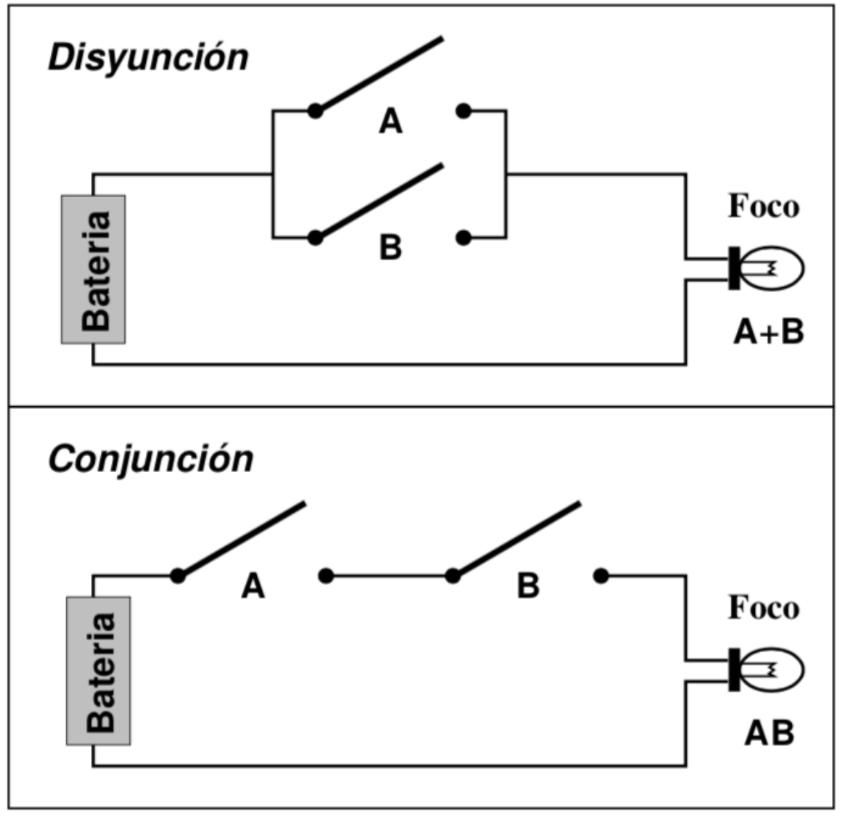
\includegraphics[width=0.5\textwidth]{image.png}
    \end{center}
    
    Escanea tu respuesta, usa un software que te ayude a modelarlo o usa alguna de las paqueterías de látex para modelar tu respuesta.
    
    \bigskip
    % -- Respuesta -- %

    \begin{center}
      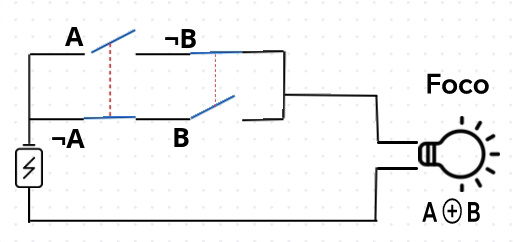
\includegraphics[width=0.8\textwidth]{image1.png}
    \end{center}
    \bigskip
\end{enumerate}
\end{document}
